\pagebreak

\section{UART CPU interface Library - xilinx/uart\_cpu.3pl}
\label{chap:lmuartcpulib}

    \index{library!xilinx/uart\_cpu.3pl}
    This library provides a CPU interface using a serial interface. This is
    by an FTDI USB port or similar.
    
    This library must be incorporated by using a {\bf module} statement -
    \begin{lstlisting}[gobble=4, language=threepl]
       module "xilinx/uart\_cpu.3pl"
    \end{lstlisting}

    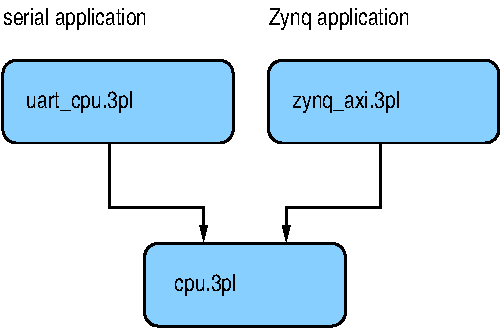
\includegraphics{cpu}

    xilinx/uart\_cpu.3pl is included in -\\
    boards/avnet/aes\_sp3a\_eval400.3pl\\
    board/gadget\_factory/papilio\_one\_100.3pl\\
    board/gadget\_factory/papilio\_one\_250.3pl\\
    board/gadget\_factory/papilio\_one\_500.3pl\\
    board/gadget\_factory/papilio\_pro\_lx4.3pl\\
    board/gadget\_factory/papilio\_pro\_lx9.3pl
    
    uart\_cpu begins by -
    
    \begin{lstlisting}[gobble=4, language=threepl]
    source "xilinx/cpu.3pl"         // CPU API classes file
    class(cpu, CPU_API());          // Create API class here as used below
    global function cpu_api () {    // Pass the API class to application code
        return(cpu);
    }
    \end{lstlisting}
    
    Since cpu.3pl is included via a source statement its code shares the scope
    of this library, UART\_CPU. Thus it can call the modules, functions and
    procedures therin.
    
    {\bf cpu.3pl} defines a class {\bf CPU\_API()} which provides the following
    class procedures for data transfer between FPGA and CPU - \\
        \hspace*{1cm}{\bf read()} generic read \autorefph{sec:lpcpurd} \\
        \hspace*{1cm}{\bf write()} generic write \autorefph{sec:lpcpuwr} \\
        \hspace*{1cm}{\bf read\_memory()} memory read \autorefph{sec:lpcpurdmem} \\
        \hspace*{1cm}{\bf read\_queue()} queue read \autorefph{sec:lpcpurdqueue} \\
        \hspace*{1cm}{\bf read\_value()} value read \autorefph{sec:lpcpurdvalue} \\
        \hspace*{1cm}{\bf write\_memory()} memory write \autorefph{sec:lpcpuwrmem} \\
        \hspace*{1cm}{\bf write\_queue()} queue write \autorefph{sec:lpcpuwrqueue} \\
        \hspace*{1cm}{\bf write\_static()} static write \autorefph{sec:lpcpuwrstat} \\
        \hspace*{1cm}{\bf dma\_read()} to FPGA from CPU \autorefph{sec:lpcpudmar} \\
        \hspace*{1cm}{\bf dma\_write()} from FPGA to CPU \autorefph{sec:lpcpudmaw} \\
        \hspace*{1cm}{\bf signal\_interrupt()} interrupt from a signal \autorefph{sec:lpcpusigint} \\
        \hspace*{1cm}{\bf interrupt()} interrupt procedure \autorefph{sec:lpcpuint} \\

    each of which can generate an instance of a CPU interface to a specific 3PL
    variable of appropriate mode. An internal class {\bf CPU\_CODEGEN} is also
    created but this is not visible to the application code 
    
    cpu.3pl is sourced by both {\bf uart\_cpu.3pl} and {\bf zynq\_axi.3pl} to
    provide CPU interfaces. The former employs a serial data link and the
    latter parallel busses.
    
    When any of the procedures above are called a defining structure is
    created which is added to a list of CPU interfaces. At the end
    of immediate execution module {\bf create\_bus\_interfaces()} is called.
    {\bf create\_bus\_interfaces()} is defined in both {\bf uart\_cpu.3pl}
    and {\bf zynq\_axi.3pl} as it is specific to each. This module
    traverses the interface list constructed above and for each interface
    calls a matching procedure in class {\bf CPU\_CODEGEN} to generate the
    logic for each instance.








    \subsection{library modules}
    



        \subsubsection{cpu\_interface - create the CPU interface low-level logic}\label{sec:lmuartcpui}

            {\bf Library: xilinx/uart\_cpu.3pl)}

            {\bf Prototype:} \\
            \vsp
            \begin{lstlisting}[gobble=12, language=threepl]
                module
                cpu_interface () {}
            \end{lstlisting}
            
            {\bf Output parameters:} \\
            
                none.                       
            
            {\bf Input parameters:} \\
            
                none.
                       
            {\bf description:} \\
            This module is called by module {\bf create\_bus\_interfaces}
            to generate the low-level interface logic to the CPU.




        \subsubsection{create\_bus\_interfaces - create the individual CPU interfaces}\label{sec:lmuartcpucbi}

            {\bf Library: xilinx/uart\_cpu.3pl)}

            {\bf Prototype:} \\
            \vsp
            \begin{lstlisting}[gobble=12, language=threepl]
                module
                create_bus_interfaces () {}
            \end{lstlisting}
            
            {\bf Output parameters:} \\
            
                none.                       
            
            {\bf Input parameters:} \\
            
                none.
                       
            {\bf description:} \\
            This module creates the logic for each of the CPU interfaces. Each
            of these communicates via logic created by module {\bf cpu\_interface}
            described above.







        \subsubsection{dma\_read - DMA read to the FPGA from CPU RAM}\label{sec:lmuartcpudmar}

            {\bf Library: xilinx/uart\_cpu.3pl)}

            {\bf Prototype:} \\
            \vsp
            \begin{lstlisting}[gobble=12, language=threepl]
                module
                dma_read (
                    queue(data)
                    <-
                    queue(address, "uint:16")   // relative memory address
                ) {}
            \end{lstlisting}
            
            {\bf Output parameters:} \\
            
                {\bf data} is the data output queue.                       
            
            {\bf Input parameters:} \\
            
                {\bf address} is a queue supplying the CPU RAM address
                relative to the DMA base address.
                       
            {\bf description:} \\
            This module performs a DMA read to the FPGA from CPU RAM. The
            transfer occurs when input queue {\bf address} is not empty
            and the output queue {\bf data} is not full.\\







        \subsubsection{dma\_write - DMA write from the FPGA to CPU RAM}\label{sec:lmuartcpudmaw}

            {\bf Library: xilinx/uart\_cpu.3pl)}

            {\bf Prototype:} \\
            \vsp
            \begin{lstlisting}[gobble=12, language=threepl]
                module
                dma_write (
                    queue(data),
                    queue(address, "uint:16")   // relative memory address
                ) {}
            \end{lstlisting}
            
            {\bf Output parameters:} \\
            
                none.                       
            
            {\bf Input parameters:} \\
                        
                {\bf data} is the data input queue.\\
                {\bf address} is a queue supplying the CPU RAM address
                relative to the DMA base address.\\
                       
            {\bf description:} \\
            This module performs a DMA write from the FPGA to CPU RAM. The
            transfer occurs when input queues {\bf address} and data are
            not empty.

        \subsubsection{sigint - interrupt the CPU on a signal}\label{sec:lmuartcpusigint}

            {\bf Library: xilinx/uart\_cpu.3pl)}

            {\bf Prototype:} \\
            \vsp
            \begin{lstlisting}[gobble=12, language=threepl]
                module
                sigint(int(n), value(sig, "log")) {}
            \end{lstlisting}
            
            {\bf Output parameters:} \\
            
                none.                       
            
            {\bf Input parameters:} \\
                        
                {\bf n} is the interrupt index, 0 to 16.\\
                {\bf sig} is a signal on whose rising edge the interrupt
                is triggered.\\
                       
            {\bf description:} \\
            When the signal {\bf sig} is asserted the interrupt is triggered.
            The interrupt number, 0 to 15, is given by {\bf index}.


    
    \subsection{library procedures}
            


        \subsubsection{add\_interface - add an interface to the interface list}\label{sec:lpuartcpuai}

            {\bf Library: xilinx/uart\_cpu.3pl)}

            {\bf Prototype:} \\
            \vsp
            \begin{lstlisting}[gobble=12, language=threepl]
                procedure
                add_interface (var(v, "->")) {}
            \end{lstlisting}
            
            {\bf Output parameters:} \\
            
                none.
                       
            {\bf Input parameters:} \\
            {\bf v} is an instance of class {\bf busCommon}, defined in
            cpu.3pl.
                     
            {\bf description:} \\
            The instance of {\bf busCommon} is added to the interface list.
            The list is processed at completion of immediate execution to
            create the whole CPU interface.


        \subsubsection{cpu\_read - write to CPU}\label{sec:lpuartcpurd}

            {\bf Library: xilinx/uart\_cpu.3pl)}

            {\bf Prototype:} \\
            \vsp
            \begin{lstlisting}[gobble=12, language=threepl]
                procedure
                cpu_read (
                    value(access, "log"),
                    value(init, "log"), 
                    queue(out)
                    <-
                    int(bus),
                    int(addr),
                    value(data_in),
                    value(contin, "log")
                ) {}
            \end{lstlisting}
            
            {\bf Output parameters:} \\
            {\bf access} is an optional output parameter which is asserted
            when a CPU to FPGA write occurs.\\
            {\bf init} is an output parameter which is asserted in the case
            of a memory read to initiate the read.\\
            {\bf out} is an optional queue variable which will be written to
            when a transfer occurs.\\

                       
            {\bf Input parameters:} \\
            {\bf bus} is not used (applies to Zynq).\\
            {\bf address} is a 6 bit interface address.\\
            {\bf data\_in} input data.\\
            {\bf contin} is only used for a memory read and is asserted
            when the memory read has occured and the transfer can begin.\\
                     
            {\bf description:} \\
            This procedure provides a low-level interface to transfer
            data from the FPGA to the CPU via the USB serial port. It is
            used by modules and procedures in library cpu.3pl and is not
            intended for use directly by application code.
            
            The CPU initiates the transfer. The transfer may consist of
            multiple bytes.


        \subsubsection{cpu\_write - write to CPU}\label{sec:lpuartcpuwr}

            {\bf Library: xilinx/uart\_cpu.3pl)}

            {\bf Prototype:} \\
            \vsp
            \begin{lstlisting}[gobble=12, language=threepl]
                procedure
                cpu_write (
                    var(out),
                    value(access, "log")
                    <-
                    int(bus),
                    int(addr)
                ) {}
            \end{lstlisting}
            
            {\bf Output parameters:} \\
            {\bf var} is a static or queue mode variable.\\          
            {\bf access} is an optional output parameter which is asserted
            when a CPU to FPGA write occurs.\\
                       
            {\bf Input parameters:} \\
            {\bf bus} is not used (applies to Zynq).\\
            {\bf address} is a 6 bit interface address.\\           
                     
            {\bf description:} \\
            This procedure provides a low-level interface to transfer
            data from the CPU to the FPGA via the USB serial port. It is
            used by modules and procedures in library cpu.3pl and is not
            intended for use directly by application code.
            
            The CPU initiates the transfer. The transfer may consist of
            multiple bytes.



    \subsection{library functions}

        \subsubsection{cpu\_api - CPU communications interface}\label{sec:lfcpuapi}

            {\bf Library: xilinx/uart\_cpu.3pl)}

            {\bf Prototype:} \\
            \vsp
            \begin{lstlisting}[gobble=12, language=threepl]
               global function
               cpu_api () {}
            \end{lstlisting}

            {\bf Return mode and type:} \\
            immediate, class

            {\bf Input parameters:} \\            
            
            none.
            
            {\bf description:} \\
            This function returns an instance of class CPU\_API












